\chapter{APK súbory}
\label{APKsubory}
APK súbory sú balíčky používané operačným systémom Android. Celý názov ukrytý za skratkou APK je \zv{Android application package file}. Tieto súbory slúžia na distribúciu aplikácií v~operačnom systéme Android. Ich použitie a význam je analogický ako pri MSI balíčkoch používaných v~systéme Microsoft Windows, alebo DEB balíčkoch používaných v~niektorých linuxových distribúciách. APK súbory sú asociované s~príponou \zv{.apk} a s~príslušným MIME typom \zv{application/vnd.android.package-archive}~\cite{Freed2016}.

Štruktúra APK balíčkov vychádza z~JAR (Java archive) balíčkov -- súborov používaných na distribúciu aplikácií alebo knižníc na platforme Java. Formát APK rozširuje všeobecnejší JAR formát o~súbory, ktoré sú špecifické pre cieľovú platformu, ktorou je operačný systém Android. Zároveň si však ponecháva vlastnosti JAR súborov. APK balíčky sú archívne súbory v~ZIP formáte. Keďže APK používajú ZIP formát, k~ich obsahu môžeme jednoducho pristúpiť rozbalením archívu štandardným spôsobom.  APK súbory vznikajú ako výstup kompletnej kompilácie a zabalenia aplikácií pre Android. APK súbor každej aplikácie obsahuje všetky potrebné súbory na jej inštaláciu a spustenie. Medzi týmito súbormi sa typicky nachádza súbor \zv{classes.dex} obsahujúci skompilovaný zdrojový kód, súbor \zv{resources.arsc} ktorý obsahuje skompilované zdroje aplikácie, súbor \zv{AndroidManifest.xml} a neskompilované súbory ako sú napríklad obrázky~\cite{buildingAndRunning}. Typická štruktúra APK balíčku je zobrazená na obrázku \ref{fig:strukturaApk}.
\begin{figure}[htb]
  \begin{center}
    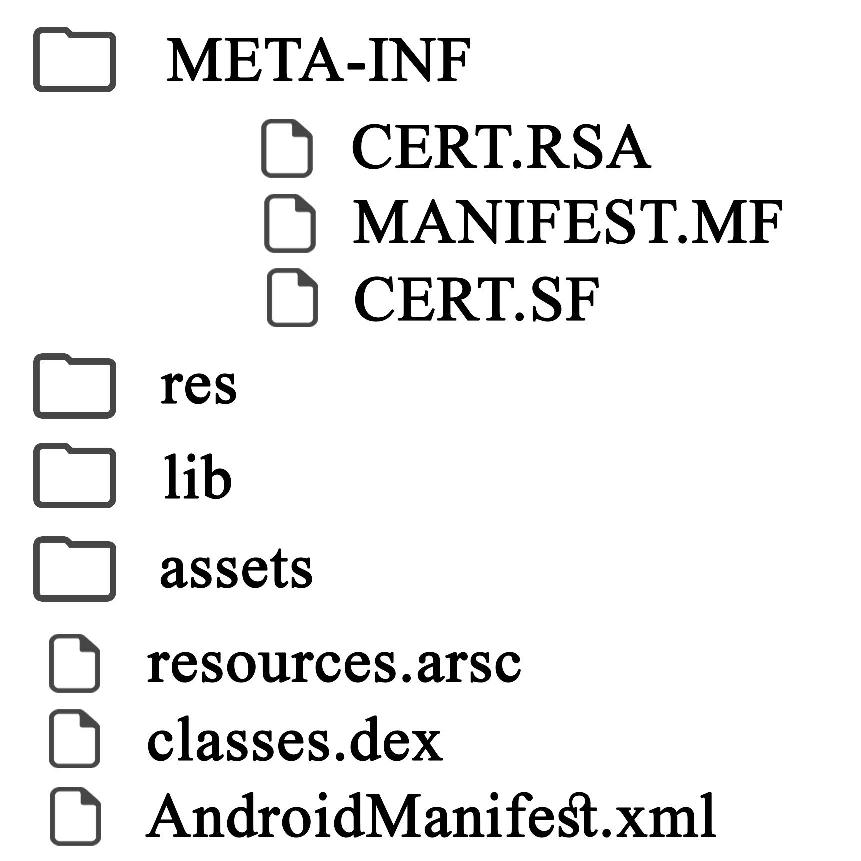
\includegraphics[width=60mm]{images/apkStructure.pdf}
  \end{center}
  \caption{Typická štruktúra APK súboru}
  \label{fig:strukturaApk}
\end{figure}
\section{Priečinok META-INF}
\label{META-INF}
Priečinok \zv{META-INF} obsahuje súbory, ktorých úlohou je zaručiť integritu ostatných súborov v~APK balíčku a s~ňou spojenú bezpečnosť celého systému. V~prípade detekcie pozmenených súborov a narušenia integrity operačný systém Android nedovolí inštaláciu APK balíčku. Po každej zmene je nutné balíček digitálne podpísať.

\subsection*{CERT.RSA}
\label{CERT.RSA} 
Súbor \zv{CERT.RSA} obsahuje verejný kľúč vo forme \zv{X509} certifikátu, ktorý slúži na overenie digitálneho podpisu balíčka.
\subsection*{MANIFEST.MF}
\label{MANIFEST.MF}
\zv{MANIFEST.MF} je súbor obsahujúci relatívne cesty a SHA-1 hashe \footnote{reťazce v~Base64 kódovaní} všetkých súborov v~APK balíčku. Tento súbor nie je špecifický len pre APK súbory, ale obsahuje ho každý JAR archív.\\\\
Typický obsah súboru \zv{MANIFEST.MF} vyzerá nasledovne~\cite{Yang2015}: \\
\begin{verbatim}
Manifest-Version: 1.0
Built-By: 0.12.2
Created-By: Android Gradle 0.12.2

Name: res/drawable-xhdpi-v4/libraries.png
SHA1-Digest: VvgaO1jpW3iS1nBBikD/urdbN58=

Name: res/layout/activity_settings.xml
SHA1-Digest: 1coP1lt9Lmccc7SMZGHxNv4bbKs=
\end{verbatim}
\subsection*{CERT.SF}
\label{CERT.SF}
Súbor \zv{CERT.SF} je podobný ako \zv{MANIFEST.MF}, avšak namiesto SHA-1 hashov samotných súborov obsahuje SHA-1 hashe záznamov o~týchto súboroch z~\zv{MANIFEST.MF}. Okrem toho obsahuje aj hash celého súboru \zv{MANIFEST.MF}. \newline Záznam o~jednom súbore v~APK balíčku v~súbore \zv{CERT.SF} vyzerá nasledovne: \newline
\begin{verbatim}
Name: res/drawable-xhdpi-v4/libraries.png
SHA1-Digest: Slg56lqothjvmaBikD/urdb7q6=
\end{verbatim}\mbox{}\\
Reťazec \zv{Slg56lqothjvmaBikD/urdb7q6=} reprezentuje SHA-1 hash nasledujúceho záznamu zo súboru \zv{MANIFEST.MF}:\mbox{}\\
\begin{verbatim}
“Name: res/drawable-xhdpi-v4/libraries.png
SHA1-Digest: VvgaO1jpW3iS1nBBikD/urdbN58=
”\end{verbatim}
\section{Priečinok res}
\label{res}
Priečinok \zv{res} obsahuje zdrojové súbory ako napríklad obrázky, zvuky alebo ikony. Okrem multimediálnych súborov obsahuje taktiež zdrojové XML súbory určujúce vzhľad obrazoviek, použité grafické štýly, alebo textové reťazce použité v~aplikácii. Niektoré z~týchto XML súborov môžu byť skompilované do binárneho formátu. V~zdrojovom kóde sú tieto zdroje odkazované pomocou unikátnych identifikátorov. Identifikátory sú generované počas kompilácie nástrojom \zv{aapt} a nachádzajú sa v~projektovej triede \zv{R}. Pre každý typ zdrojového súboru je generovaná podtrieda triedy \zv{R}~\cite{accessingRes}. Všetky zdroje aplikácie by mali byť externalizované a uložené v~špecifickom podpriečinku v~tomto adresári. \newpage
\textbf{Podporované podpriečinky}~\cite{providingRes}
\begin{itemize}
\item animator - obsahuje XML súbory definujúce property animácie\footnote{Animácie definované pomocou zmeny atribútov vykreslovaných objektov},
\item anim - obsahuje XML súbory definujúce tween animácie\footnote{Animácie definované pomocou štartového bodu, koncového bodu, rotáciou a inými transformáciami vykreslovaného objektu}, môže obsahovať aj property animácie,
\item color - obsahuje XML súbory definujúce farby a ich zmeny na základe stavu objektov na ktoré sú aplikované,
\item drawable - obsahuje obrázky vo formáte PNG, 9.PNG, JPG, GIF alebo XML súbory skompilované do formy vykresliteľných obrázkov,
\item mipmap - obsahuje ikony aplikácie s~rôznou hustotou pixelov,
\item layout - obsahuje súbory vo formáte XML definujúce vzhľad a rozmiestnenie prvkov na obrazovke,
\item menu - obsahuje XML súbory definujúce menu aplikácie,
\item raw - obsahuje súbory, ktoré musia byť uložené a použité v~neskomprimovanej forme a kvalite,
\item values - obsahuje súbory vo formáte XML definujúce hodnoty textových reťazcov, farieb, štýlov alebo základných rozmerov,
\item xml - obsahuje XML súbory, ktoré môžu byť načítané počas behu aplikácie.
\end{itemize}

\noindent V~spomenutých priečinkoch sú uložené základné zdroje aplikácie. Tieto zdrojové súbory určujú základný dizajn a obsah aplikácie. Rôzne typy Android zariadení môžu využívať rôzne zdrojové súbory. Alternatívne zdroje sa využívajú na prispôsobenie dizajnu a obsahu veľkosti a aktuálnej konfigurácií zariadenia. Sú umiestnené v~priečinku, ktorého názov pozostáva z~typu zdrojového súboru, ktorý korešponduje so základným názvom priečinku a názvu hodnoty konfiguračného atribútu pre ktorý je tento priečinok určený. Je možné kombinovať viacero konfiguračných atribútov~\cite{providingAltRes}.\\\\
\textbf{Najčastejšie používané atribúty}
\begin{itemize}
\item Jazyk a región – jazyk je definovaný podľa kódovania \zv{ISO 639-1}~\cite{isoCodes} s~možnosťou rozšírenia pomocou \zv{ISO 3166-1-alpha-2} regionálneho kódu. Napríklad obrázky špecifické pre zariadenia s~francúzskym jazykom sa nachádzajú v~priečinku \cesta{res/drawable-fr}.
\item Veľkosť obrazovky –  v~závislosti na veľkosti a rozlíšení obrazovky rozlišuje štyri možné hodnoty -- \zv{small}, \zv{normal}, \zv{large}, \zv{xlarge}.
\item Orientácia obrazovky – umožňuje definovať rôzne zdrojové súbory v~závislosti na orientácii zariadenia. Hodnota \zv{port} špecifikuje súbory pre zariadenie orientované vertikálne, hodnota \zv{land} je určená pre horizontálnu orientáciu zariadenia.	
\item Hustota obrázkových bodov obrazovky -  hodnoty určujúce vhodnosť zdrojových súborov vzhľadom na hustotu obrázkových bodov obrazovky daného zariadenia.
\end{itemize}


\section{Priečinok lib}
\label{lib}
Priečinok \zv{lib} obsahuje skompilovaný zdrojový kód natívnych knižníc. Tieto knižnice sú špecifické pre typ a architektúru procesora. V~závislosti na architektúre procesora obsahuje podpriečinky: \zv{armeabi}, \zv{armeabi-v7a}, \zv{arm64-v8a}, \zv{x86}, \zv{x86\_64}, \zv{mips}.

\section{Priečinok assets}
\label{assets}
Priečinok \zv{assets} obsahuje súbory uložené a používané v~originálnej neskomprimovanej forme. V~tomto priečinku sa často nachádzajú textové súbory, HTML súbory, licenčné informácie, obrázky alebo textúry. Na rozdiel od priečinku \cesta{res/raw/}, zdrojovým súborom v~umiestneným v~priečinku \zv{assets} nie sú pridelené unikátne identifikátory uložené v~triede \zv{R.java}. K~súborom sa pristupuje ako k~dátam uloženým v~bežnom súborovom systéme. Trieda \zv{AssetManager} poskytuje funkcionalitu na čítanie súborov ako prúdu bytov a navigáciu v~tomto priečinku~\cite{AssetManager}.

\section{resources.arsc}
\label{resources.arsc}
Súbor \zv{resources.arsc} obsahuje mapovanie medzi zdrojovými súbormi  z~priečinku \zv{res} a ich identifikátormi.  Vytvára sa počas kompilácie. Obsahuje XML súbory v~binárnom formáte.

\section{classes.dex}
\label{classes.dex}
\zv{Classes.dex} je súbor obsahujúci skompilovaný zdrojový kód aplikácie.  Zdrojové súbory Android aplikácií sú napísané v~jazyku Java. Java súbory sú skompilované do Java bytekódu pomocou bežného kompilátoru pre platformu Java. Výsledkom tejto kompilácie sú súbory s~príponou \zv{.class}, ktoré sú následne preložené do \zv{Dalvik} bytekódu pomocou nástroja \zv{dx}, ktorý je súčasťou \zv{Android SDK}~\cite{Reddy2014}. Výstupom nástroju \zv{dx} je jediný súbor obsahujúci skompilovaný celý výkonný zdrojový kód aplikácie -- \zv{classes.dex}. Tento súbor je skomprimovanou a optimalizovanou verziou všetkých \zv{.class} súborov~\cite{Georgiev2014}. Takto skompilovaný program môže byť vykonaný len vo virtuálnom stroji \zv{Dalvik}, alebo v~novšom prostredí \zv{ART (Android Runtime)} používanom primárne od verzie \zv{Android 5.0 Lollipop}~\cite{dalvik}.

\section{AndroidManifest.xml} 
\label{AndroidManifest.xml}
\zv{AndroidManifest.xml} je súbor, ktorý musí obsahovať každá aplikácia. Tento súbor poskytuje informácie o~aplikácii operačnému systému Android. Neobsahuje žiadny výkonný kód. Definuje meno a verziu, ktoré slúžia ako unikátny identifikátor danej aplikácie. Popisuje všetky komponenty z~ktorých sa aplikácia skladá, cesty k~použitým knižniciam, minimálny vyžadovaný level Android API, oprávnenia vyžadované aplikáciou na prístup k~chráneným častiam Android API a taktiež oprávnenia, ktoré sú vyžadované od iných komponent pri pokuse komunikovať s~danou aplikáciou~\cite{appManifest}. Súbor \zv{AndroidManifest.xml}, ktorý nájdeme v~APK balíčku je vo formáte binárneho XML súboru. Je ho však možné previesť do klasického čitateľného XML formátu.

Keďže \zv{AndroidManifest.xml} je základným súborom poskytujúcim metadáta o~Android aplikácii a APK súbore, informácie získané z~tohto súboru tvoria veľkú časť štatistických dát zbieraných a vyhodnocovaných v~kapitole \ref{statistiky}. Preto sa detailnejšie pozrieme na jeho štruktúru a niektoré dôležité elementy, ktoré obsahuje.
\begin{lstlisting} [language=XML, caption= {Základná štruktúra súboru /AndroidManifest.xml}]*<manifest>
    <uses-permission />
    <permission />
    <uses-sdk />
    <uses-configuration />  
    <uses-feature />  
    <supports-screens />  
    <compatible-screens />  
    <application>
        <activity />
        <service/>
        <receiver/>
        <provider/>
        <uses-library />
    </application>
</manifest>
\end{lstlisting}

\subsection{Element manifest}
\label{el_manifest}
\lstset{language=XML}
\begin{lstlisting}
<manifest xmlns:android="URL"
          package="string"
          android:sharedUserId="string"
          android:sharedUserLabel="string resource"
          android:versionCode="integer"
          android:versionName="string"
          android:installLocation=["auto" | "internalOnly" |
                                        "preferExternal"] >
</manifest>
\end{lstlisting}
\zv{AndroidManifest.xml} obsahuje element \zv{manifest} ako koreňový prvok. Tento element je povinný a každý súbor \zv{AndroidManifest.xml} ho obsahuje práve jeden. \newline\newline
\noindent Element \zv{manifest} definuje atribúty~\cite{elManifest}:\\
\begin{itemize}
\item \bod{xmlns:android} -- povinný atribút definujúci menný priestor,
\item \bod{package} -- nemenný názov balíku aplikácie, povinný atribút definujúci identitu aplikácie,
\item \bod{android:sharedUserId} -- identifikátor aplikácie zdieľaný s~ostatnými aplikáciami za účelom vzájomnej komunikácie,
\item \bod{android:sharedUserLabel} -- čitateľná podoba \zv{android:sharedUserId} identifikátoru,
\item \bod{android:versionCode} -- interná informácia o~verzii aplikácie. Tento atribút je využívaný len na rozoznanie novších verzií od starších. Novšie aplikácie obsahujú vyššiu hodnotu,
\item \bod{android:versionName} –- informácia o~verzii aplikácie prezentovaná užívateľom. Pre systém Android neposkytuje informáciu o~verzii, tú obsahuje atribút \zv{android:versionCode},
\item \bod{android:installLocation} – určuje predvolené umiestnenie inštalácie aplikácie. Pokiaľ je aplikáciu možné nainštalovať len do vnútornej pamäti zariadenia, obsahuje hodnotu \zv{internalOnly}. Takáto aplikácia nemôže byť presunutá na externé pamäťové médium (typicky SD karta). Táto hodnota sa použije v~prípade, že tento atribút nie je definovaný. V~prípade hodnoty \zv{auto} sú aplikácie inštalované do vnútornej pamäti, ale môžu byť presunuté do pamäti externej. Hodnota \zv{preferExternal} zabezpečí, že systém sa pokúsi o~inštaláciu na externé pamäťové médium. V~prípade neúspechu sa použije interná pamäť.
\end{itemize}

\subsection{Element uses-permission}
\label{el_uses-permission}
\lstset{language=XML}
\begin{lstlisting}
<uses-permission android:name="string"
        android:maxSdkVersion="integer" />
\end{lstlisting}
Prístup k~niektorým dátam alebo funkciám Andorid API je z~dôvodu ochrany limitovaný. Android využíva princíp povolení\footnote{angl. permissions}. Povolenia môžu byť definované samotnou aplikáciou, inou aplikáciou alebo systémom Android. Aplikácia, ktorá chce pristupovať k~chráneným dátam alebo používať chránené časti kódu, musí pomocou elementu \zv{uses-permissions} deklarovať vyžadovaný prístup k~chráneným častiam~\cite{appManifest}. Prístupové povolenia sú aplikácii schválené užívateľom. Vo verzii Android 5.1 a starších, systém počas inštalácie oboznámi užívateľa so všetkými povoleniami, ktoré aplikácia vyžaduje. V~prípade, že ich používateľ neschváli, aplikácia nebude nainštalovaná. Od verzie Android 6.0 užívateľ schvaľuje povolenia počas behu aplikácie.\\\\ 
Element \zv{uses-permission} definuje atribúty~\cite{elUsesPerm}:\\
\begin{itemize}
\item \bod{android:name} -- názov povolenia,
\item \bod{android:maxSdkVersion} -- najvyšší level Android API, pre ktorý je dané povolenie potrebné.
\end{itemize}

\subsection{Element permission}
\lstset{language=XML}
\begin{lstlisting}
<permission android:description="string resource"
            android:icon="drawable resource"
            android:label="string resource"
            android:name="string"
            android:permissionGroup="string"
            android:protectionLevel=["normal"|"dangerous"| 
                                     "signature"|
                                     "signatureOrSystem"] />
\end{lstlisting}
Definuje bezpečnostné povolenie, ktoré môže byť použité na obmedzenie prístupu ku komponente aplikácie. Toto povolenie je následne používané aplikáciami, ktoré vyžadujú prístup k~chránenej časti poskytovanej danou aplikáciou.\\\\ Najdôležitejšie atribúty definované v~rámci elementu \zv{permission}~\cite{elPerm}:\\
\begin{itemize}
\item \bod{android:name} -- názov povolenia, aplikácie vyžadujúce dané povolenie uvádzajú túto hodnotu v~atribúte, \zv{android:name} v~tagu \zv{uses-permission}. Názov musí byť unikátny a mal by dodržiavať menné konvencie jazyka Java,
\item \bod{android:permissionGroup} -- priradí toto povolenie do skupiny povolení. Táto skupina povolení musí byť deklarovaná v~rámci elementu \zv{permission-group} v~niektorej z~nainštalovaných aplikácií. Slúži na logické zoskupenie významovo podobných oprávnení,
\item \bod{android:protectionLevel} -- charakterizuje potenciálne riziko spojené s~použitím daného povolenia. Táto hodnota určuje postup operačného systému pri rozhodovaní o~udelení povolenia. 
Základnou hodnotou je \zv{normal}, ktorý reprezentuje povolenia s~nízkou mierou rizika. Tieto povolenia sú aplikácii automaticky schválené systémom Android počas inštalácie. Pre povolenia so~zvýšenou mierou rizika je určená hodnota \zv{dangerous}. Tieto povolenia typicky udeľujú aplikácii prístup k~citlivým dátam alebo k~prvkom zariadenia, ktoré môžu negatívne ovplyvniť jeho používanie. Pretože tento typ povolení prináša potenciálne riziko, systém ho nemôže udeliť automaticky, ale až po explicitnom súhlase používateľa.
V~prípade, že tento atribút obsahuje hodnotu \zv{signature}, povolenie je udelené automaticky a to len aplikáciám, ktorých certifikát je rovnaký ako certifikát aplikácie definujúcej dané povolenie.   
Hodnota \zv{signatureOrSystem} rozširuje hodnotu \zv{signature} a povolenia sú udelené aj aplikáciám typu \zv{Android system image}.
\end{itemize}

\subsection{Element uses-sdk}
\lstset{language=XML}
\begin{lstlisting}
<uses-sdk android:minSdkVersion="integer"
          android:targetSdkVersion="integer"
          android:maxSdkVersion="integer" />
\end{lstlisting}
Element vyjadrujúci kompatibilitu aplikácie s~verziou Androidu pomocou čísla verzie Android API.\\\\
Atribúty definované elementom \zv{uses-sdk}~\cite{elUsesSdk}:\\
\begin{itemize}
\item \bod{android:minSdkVersion} -- vyjadruje najnižší level API vyžadovaný aplikáciou. Pokiaľ je táto hodnota vyššia ako API úroveň zariadenia, systém zabráni inštalácii. Tento atribút by mala obsahovať každá aplikácia,
\item \bod{android:targetSdkVersion} -- informuje o~úrovni API na ktorej bola aplikácia testovaná a pre ktorú je primárne určená. V~prípade, že zariadenie podporuje vyššiu verziu Android API ako definuje spomínaný atribút, aplikácia môže byť spustená v~móde kompatibility s~touto verziou API,
\item \bod{android:maxSdkVersion} -- najvyššia úroveň API kompatibilná s~aplikáciou. Z~dôvodu spätnej kompatibility nie je používanie tohto atribútu doporučené. Tento atribút bol využívaný len do verzie Android 2.0.1.
\end{itemize}

\subsection{Element uses-feature}
\label{el_uses-feature}
\lstset{language=XML}
\begin{lstlisting}
<uses-feature
  android:name="string"
  android:required=["true" | "false"] />
\end{lstlisting}
Deklaruje hardvérovú alebo softvérovú vlastnosť \footnote{angl. feature} používanú aplikáciou. Tento element informuje externé entity o~funkciách, ktoré aplikácia vyžaduje. Deklarované vlastnosti majú informačný charakter. Systém Android nekontroluje, či zariadenie podporuje všetky vlastnosti deklarované aplikáciou. Tento element je využívaný službou \zv{Google Play} na  filtrovanie aplikácií vyhovujúcich danému zariadeniu, a preto by mala byť deklarovaná každá vyžadovaná vlastnosť.\\\\ Element obsahuje nasledujúce atribúty~\cite{elUsesFeature}:\\
\begin{itemize}
\item \bod{android:name} -- názov vyžadovanej vlastnosti,
\item \bod{android:required} -- určuje, či aplikácia vyžaduje danú vlastnosť pre korektné fungovanie. Pokiaľ obsahuje hodnotu \zv{true}, aplikácia nie je schopná korektne fungovať na zariadení nepodporujúcom danú vlastnosť.
\end{itemize}

\subsection{Element supports-screens}
\lstset{language=XML}
\begin{lstlisting}
<supports-screens android:resizeable=["true"| "false"]
                  android:smallScreens=["true" | "false"]
                  android:normalScreens=["true" | "false"]
                  android:largeScreens=["true" | "false"]
                  android:xlargeScreens=["true" | "false"]
                  android:anyDensity=["true" | "false"]
                  android:requiresSmallestWidthDp="integer"
                  android:compatibleWidthLimitDp="integer"
                  android:largestWidthLimitDp="integer"/>
\end{lstlisting}
Špecifikuje podporované typy obrazoviek. V~prípade inštalácie na zariadení s~väčšou obrazovkou ako aplikácia podporuje, informuje systém o~potrebe využitia módu obrazovej kompatibility.\\\\ Väčšina atribútov deklaruje podporované veľkosti obrazoviek. Medzi ostatné atribúty definované elementom \zv{supports-screens} patria~\cite{elScreen}:\\
\begin{itemize}
\item \bod{android-resizeable} -- indikuje schopnosť aplikácie korektne sa prispôsobiť rôznym veľkostiam obrazoviek,
\item \bod{android:anyDensity} -- indikuje, že aplikácia obsahuje zdrojové súbory vhodné pre obrazovky s~rôznou hustotu obrazových bodov.
\end{itemize}

\subsection{Element activity}
\label{el_activity}
Deklaruje aktivity. Aktivity sú základnými časťami aplikácie. Sú to triedy rozširujúce triedu \zv{android.app.Activity}. Sú zamerané na jednotlivé prípady použitia aplikácie, implementujú časť grafického užívateľského rozhrania a zabezpečujú komunikáciu s~užívateľom. Tieto triedy sú časťou zdrojového kódu a v~skompilovanej forme sa nachádzajú v~súbore \zv{classes.dex} (viď \ref{classes.dex}). Pri viacerých spustených aktivitách zohráva dôležitú úlohu životný cyklus aktivity~\cite{elActivity}. Všetky aktivity musia byť deklarované pomocou elementu \zv{activity}. V~prípade, že deklarované nie sú, systém ich ignoruje a nebudú spustené.

\subsection{Element service}
Deklaruje komponenty aplikácie typu služba\footnote{angl. service}. Na rozdiel od aktivít, služby nemajú grafické používateľské rozhranie. Slúžia na implementáciu dlhodobých úloh na pozadí, ktoré môžu byť spustené aj v~čase keď aplikácia nie je aktívna na popredí. 
Služby implementujú funkcionalitu využívanú aplikáciou. Rozlišujeme dva typy služieb~\cite{elService}. Služby typu \zv{started} po spustení bežia pokým nedokončia svoju úlohu a ostatným komponentom nevracajú výsledok. Služby typu \zv{bound} komunikujú s~ostatnými komponentami pomocou modelu klient-server a sú ukončené keď pre nich neexistuje klient~\cite{boundService}. Každá služba rozširuje základnú triedu \zv{android.app.Service} a musí byť deklarovaná pomocou elementu \zv{service}, inak bude ignorovaná.

\subsection{Element provider}
Deklaruje komponenty aplikácie, ktorých úlohou je poskytovanie štrukturovaného prístupu k~dátam spravovaným aplikáciou. Poskytovatelia obsahu\footnote{angl. content providers} sú implementovaní ako podtriedy triedy \zv{ andro\-id.con\-tent.Con\-tent\-Pro\-vi\-der}. Využitie tejto komponenty je nutné len v~prípade potreby zdieľania dát medzi viacerými aplikáciami. Operačný systém Android si ukladá referencie na jednotlivých poskytovateľov obsahu pomocou \zv{authority} textového reťazca, ktorý je definovaný ako jeden z~atribútov elementu \zv{provider}~\cite{elContentProvider}. Systém Android nerozpoznáva poskytovateľov obsahu nedefinovaných v~\zv{AndroidManifest.xml}.

\subsection{Element receiver}
Deklaruje komponentu aplikácie implementovanú ako podtriedu triedy \zv{android.content.BroadcastReceiver}. Tieto komponenty umožňujú aplikácii prijímať a reagovať na informácie o~zámere spustenia aktivity\footnote{Intent} aj v~čase, keď ostatné komponenty aplikácie nie sú spustené. Systém Android môžeme oboznámiť s~existenciou komponent tohto typu pomocou elementu \zv{receiver} v~súbore \zv{AndroidManifest.xml} alebo aj dynamicky pomocou volania \zv{Context.registerReceiver()} v~zdrojovom kóde aplikácie~\cite{elReceiver}.

\subsection{Element uses-library}
\lstset{language=XML}
\begin{lstlisting}
<uses-library
  android:name="string"
  android:required=["true" | "false"] />
\end{lstlisting}
Špecifikuje zdieľanú knižnicu vyžadovanú aplikáciou. Tento element informuje systém o~potrebe zahrnúť cestu k~zdrojovému kódu knižnice medzi cesty v~ktorých \zv{Dalvik Virtual Machine} hľadá zdrojové súbory. V~angličtine sú tieto cesty označované ako \zv{class path}. Balíky, ktoré sú v~Android aplikáciách najpoužívanejšie, napríklad \zv{android.app}, \zv{android.content} alebo \zv{android.view} sú obsiahnuté v~základnej knižnici, ktorá je automaticky pripojená ku každej aplikácií a nemusí byť deklarovaná týmto elementom. Balíčky, ktoré nie sú medzi základnými knižnicami, musia byť deklarované.  Tento element ovplyvňuje inštaláciu aplikácie na konkrétnom zariadení a taktiež dostupnosť aplikácie v~obchode \zv{Google Play}.\\\\ Definuje atribúty~\cite{elUsesLib}:\\
\begin{itemize}
\item \bod{android:name} -- názov knižnice, ktorý sa nachádza v~dokumentácii príslušného použitého balíčku,
\item \bod{android:required} -- indikuje či aplikácia nevyhnutne vyžaduje knižnicu špecifikovanú atribútom \zv{android:name}. V~prípade hodnoty \zv{true} aplikácia nie je schopná fungovať bez danej knižnice. Systém zamietne inštaláciu takejto aplikácie, pokiaľ zariadenie neobsahuje danú knižnicu. Ak je tento atribút nastavený na hodnotu \zv{false}, aplikácia je schopná korektne fungovať aj bez danej knižnice.
\end{itemize}